\documentclass[11pt]{article}

\usepackage[margin=1in]{geometry}
\usepackage[T1]{fontenc}
\usepackage{lmodern}
\usepackage{microtype}
\usepackage{amsmath,amssymb}
\usepackage{booktabs}
\usepackage{graphicx}
\usepackage{xcolor}
\usepackage[numbers,sort&compress]{natbib}
\usepackage{tikz}
\usetikzlibrary{positioning,arrows.meta,fit,calc}
\usepackage[colorlinks=true,linkcolor=blue!60!black,citecolor=blue!60!black,urlcolor=blue!60!black]{hyperref}
\usepackage{cleveref}

\newcommand{\tok}[1]{\texttt{<#1>}}

\title{\textbf{Hale-VLA: An Interleaved Vision--Language--Action Transformer\\with DeepSeek-Style Mixture-of-Experts, Built From Scratch}}
\author{B A NaveenKumar\\
\small Independent researcher\\
\small \url{https://github.com/basaanithanaveenkumar/Hale-VLA}}
\date{}

\begin{document}
\maketitle

\begin{abstract}
Vision--language--action (VLA) models extend multimodal language models so that the same
network that describes a scene can also emit robot actions. Most open VLAs are built by
fine-tuning a large pretrained vision--language model, which makes the architecture hard to
inspect and expensive to modify. We present \textbf{Hale-VLA}, a compact VLA written from
scratch in PyTorch whose every component---patch encoder, causal decoder, mixture-of-experts
feed-forward layers, proprioceptive state encoder and continuous action head---fits in a few
hundred lines of readable code. Hale-VLA represents images, robot state and actions as three
special tokens (\tok{image}, \tok{state}, \tok{action}) added to the Qwen2.5 vocabulary, so
arbitrary interleavings of observations, dialogue and control can be expressed as a single
chat transcript. Image patches are prepended to the sequence, state vectors are injected in
place of their placeholder tokens, and action predictions are read out from the decoder's
hidden states at \tok{action} positions and decoded into action chunks by an MLP. Each decoder
block uses a DeepSeekMoE-style layer with always-on shared experts and noisy top-$k$ routed
SwiGLU experts. The default configuration has 356M parameters, of which roughly 58M decoder
parameters are active per token. The model is trained end-to-end with next-token
cross-entropy on assistant turns plus a masked regression loss on actions, using the
interleaved and question-answering subsets of EO-Data1.5M. We describe the design, its data
pipeline and training objective, and release the full implementation as a testbed for VLA
architecture research.
\end{abstract}

\section{Introduction}

Large vision--language models (VLMs) have become the default starting point for generalist
robot policies. RT-2~\cite{brohan2023rt2} showed that co-fine-tuning a web-scale VLM on robot
trajectories, with actions written as text tokens, transfers semantic knowledge to control.
OpenVLA~\cite{kim2024openvla} made this recipe open, and $\pi_0$~\cite{black2024pi0} replaced
token-discretised actions with a flow-matching action expert. More recently,
EO-1~\cite{qu2025eo1} argued that \emph{interleaving} vision, text and action in one sequence
during pretraining improves embodied reasoning, and released the EO-Data1.5M corpus to
support it.

These systems share a practical drawback: they inherit billions of parameters and a large
external codebase from the underlying VLM. Answering simple architectural
questions---\emph{where should proprioception enter the sequence? does sparse routing help
action prediction? how should action chunks be read out?}---requires changes deep inside
code that was not written for them.

Hale-VLA takes the opposite approach. It is a small VLA in which every module is written
from first principles, while still speaking the same interface as larger systems: a
Qwen2.5~\cite{qwen2025qwen25} tokenizer, a chat template, multi-image interleaved inputs and
chunked continuous actions. Our contributions are:
\begin{itemize}
  \item A \textbf{unified token interface} for VLAs with three special tokens and three
        integration patterns---\emph{prepend} (images), \emph{in-place injection}
        (state) and \emph{hidden-state read-out} (actions)---that together support
        arbitrary interleavings of observations, language and control (\cref{sec:tokens}).
  \item A \textbf{from-scratch MoE decoder} combining DeepSeekMoE~\cite{dai2024deepseekmoe}
        shared experts with noisy top-$k$ gating~\cite{shazeer2017outrageously} and SwiGLU
        experts~\cite{shazeer2020glu} (\cref{sec:moe}).
  \item A \textbf{joint objective and data pipeline} for EO-Data1.5M that masks non-assistant
        turns and pads images, states and action chunks per batch (\cref{sec:training}).
  \item An open, test-friendly implementation with measured parameter budgets
        (\cref{tab:params}) intended as a baseline for architecture ablations.
\end{itemize}

\section{Related Work}

\paragraph{Vision--language models.} LLaVA~\cite{liu2023llava} popularised connecting a
vision encoder~\cite{dosovitskiy2021vit} to a language model through a learned projector and
training on instruction data. Hale-VLA follows the same encoder--projector--decoder layout
but trains the vision tower jointly rather than freezing a CLIP encoder.

\paragraph{Vision--language--action models.} RT-2~\cite{brohan2023rt2} and
OpenVLA~\cite{kim2024openvla} discretise actions into vocabulary tokens. Octo~\cite{octo2024}
and $\pi_0$~\cite{black2024pi0} use continuous action heads (diffusion and flow matching).
ACT~\cite{zhao2023aloha} introduced predicting \emph{chunks} of future actions to reduce
compounding error. Hale-VLA uses a continuous MLP head that predicts action chunks from the
hidden state of an \tok{action} token, keeping the language model's vocabulary free of
action bins. Large cross-embodiment datasets such as Open X-Embodiment~\cite{oxe2023} and
EO-Data1.5M~\cite{qu2025eo1} make joint training of reasoning and control possible.

\paragraph{Mixture-of-experts.} Sparsely gated MoE layers~\cite{shazeer2017outrageously}
increase capacity at constant per-token compute. DeepSeekMoE~\cite{dai2024deepseekmoe} adds
\emph{shared} experts that every token uses, so routed experts can specialise. We adopt this
design inside both the decoder and the vision encoder.

\section{Method}

\begin{figure}[t]
\centering
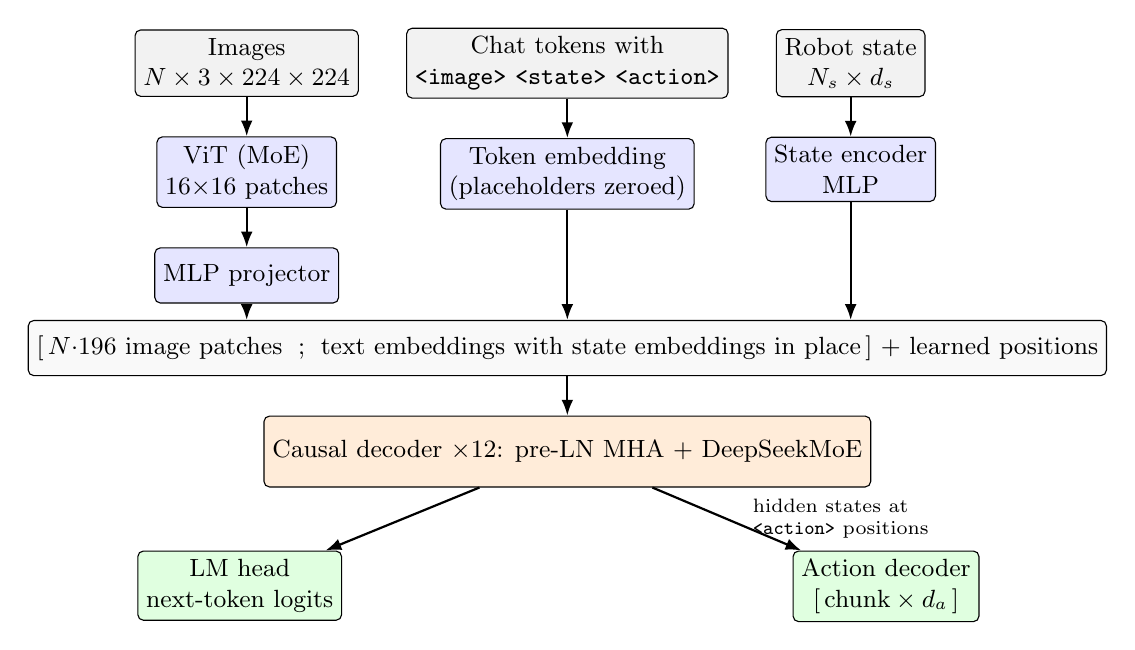
\begin{tikzpicture}[
  node distance=5mm and 6mm,
  box/.style={draw, rounded corners=2pt, align=center, font=\small, minimum height=7mm, inner sep=3pt},
  inp/.style={box, fill=gray!10},
  enc/.style={box, fill=blue!10},
  core/.style={box, fill=orange!15, minimum width=62mm, minimum height=9mm},
  head/.style={box, fill=green!12},
  arr/.style={-{Latex[length=2mm]}, thick}
]
\node[inp] (img) {Images\\$N\times3\times224\times224$};
\node[inp, right=of img] (txt) {Chat tokens with\\\tok{image} \tok{state} \tok{action}};
\node[inp, right=of txt] (st) {Robot state\\$N_s\times d_s$};

\node[enc, below=of img] (vit) {ViT (MoE)\\16$\times$16 patches};
\node[enc, below=of vit] (proj) {MLP projector};
\node[enc, below=of txt] (emb) {Token embedding\\(placeholders zeroed)};
\node[enc, below=of st] (senc) {State encoder\\MLP};

\node[box, below=14mm of emb, minimum width=118mm, fill=gray!5] (seq) {[\,$N{\cdot}196$ image patches \;;\; text embeddings with state embeddings in place\,] + learned positions};
\node[core, below=of seq] (dec) {Causal decoder $\times12$: pre-LN MHA + DeepSeekMoE};
\node[head, below left=8mm and -10mm of dec] (lm) {LM head\\next-token logits};
\node[head, below right=8mm and -10mm of dec] (act) {Action decoder\\$[\,\text{chunk}\times d_a\,]$};

\draw[arr] (img) -- (vit);
\draw[arr] (vit) -- (proj);
\draw[arr] (txt) -- (emb);
\draw[arr] (st) -- (senc);
\draw[arr] (proj) -- (proj |- seq.north);
\draw[arr] (emb) -- (seq);
\draw[arr] (senc) -- (senc |- seq.north);
\draw[arr] (seq) -- (dec);
\draw[arr] (dec) -- (lm);
\draw[arr] (dec) -- node[right=2mm, font=\scriptsize, align=left]{hidden states at\\\tok{action} positions} (act);
\end{tikzpicture}
\caption{Hale-VLA. Images are encoded by a patch transformer and prepended; state vectors
replace their \tok{state} placeholders in place; hidden states at \tok{action} positions are
decoded into continuous action chunks.}
\label{fig:arch}
\end{figure}

\subsection{Token interface}
\label{sec:tokens}

We extend the Qwen2.5 tokenizer~\cite{qwen2025qwen25} (151{,}643 base tokens) with three
special tokens: \tok{image} (id 151665), \tok{action} (151666) and \tok{state} (151667),
giving a vocabulary of $V=151{,}668$. Every training sample is rendered as a chat transcript
with a system prompt, user turn and assistant turn, and the special tokens appear wherever
the corresponding modality occurs. Given input ids $x_{1:L}$, the model builds its input
sequence with three patterns.

\paragraph{Prepend (images).} For each of the $N$ images in a sample, the vision encoder
produces $P=(224/16)^2=196$ patch features, which a three-layer MLP projector
(Linear--LN--GELU twice, then Linear, widths $d/4 \to d/2 \to d$) maps to the decoder width
$d=512$. All $N\cdot P$ projected patches are concatenated \emph{before} the text sequence,
so every text token can attend to all visual context under the causal mask.

\paragraph{In-place injection (state).} Each proprioceptive vector $s_j\in\mathbb{R}^{d_s}$
is encoded by an MLP ($d_s\to256\to512\to d$ with LayerNorm, GELU and dropout) into a single
embedding that overwrites the $j$-th \tok{state} position. States therefore stay at their
temporal location in the dialogue, which matters for interleaved trajectories where several
observations and states alternate.

\paragraph{Read-out (actions).} \tok{action} tokens are embedded like ordinary tokens. After
the decoder, their hidden states (offset by the $N\cdot P$ prepended positions) are passed to
the action decoder. Because the read-out position sees all preceding images, states and
instructions, the \tok{action} token acts as a learned query that summarises the context
into a control command.

Placeholder embeddings for \tok{image} and \tok{state} are zeroed before injection, and a
learned absolute position embedding (up to 2{,}000 positions) is added to the full combined
sequence.

\subsection{Vision encoder}

The vision encoder is a ViT~\cite{dosovitskiy2021vit}: a $16{\times}16$ convolutional patch
embedding, learned positional embeddings, four pre-norm transformer blocks with 16 heads and
a final LayerNorm. Its feed-forward layers are the same DeepSeekMoE layers as the decoder
(16 routed experts, top-4, two shared experts), giving the vision tower high capacity at
moderate compute. It is trained from scratch jointly with the rest of the model.

\subsection{Decoder with DeepSeek-style MoE}
\label{sec:moe}

The decoder stacks 12 pre-LayerNorm~\cite{xiong2020layer} blocks,
\begin{align}
  h' &= h + \mathrm{MHA}_{\text{causal}}(\mathrm{LN}_1(h)), &
  h'' &= h' + \mathrm{MoE}(\mathrm{LN}_2(h')),
\end{align}
with 16 attention heads of width 32. Each MoE layer contains $S=2$ shared experts and $E=8$
routed experts. Every expert is a SwiGLU~\cite{shazeer2020glu} MLP,
$\mathrm{FFN}_e(u)=W_2^{e}\big(\mathrm{SiLU}(W_1^{e}u)\odot W_3^{e}u\big)$, with hidden width
$\mathrm{round}(1.2d)=614$. Routing uses noisy top-$k$ gating~\cite{shazeer2017outrageously}:
\begin{align}
  g(u) &= W_g u + \epsilon\odot\mathrm{softplus}(W_n u),\quad \epsilon\sim\mathcal N(0,I)\ \text{(training only)},\\
  p(u) &= \mathrm{softmax}\big(\mathrm{TopK}(g(u),k)\big),\qquad k=2,\\
  \mathrm{MoE}(u) &= \sum_{s=1}^{S}\mathrm{FFN}^{\text{sh}}_{s}(u) + \sum_{e\in\mathrm{TopK}} p_e(u)\,\mathrm{FFN}_e(u),
\end{align}
where $\mathrm{TopK}$ sets non-selected logits to $-\infty$. Shared experts capture common
transformations for all tokens, letting routed experts specialise, e.g.\ by modality or
task. A final LayerNorm and a linear LM head produce next-token logits over all
$N\cdot P+L$ positions.

\subsection{Action decoder}

The action decoder maps each read-out hidden state $h_a\in\mathbb{R}^{d}$ to an action chunk
$\hat a\in\mathbb{R}^{C\times d_a}$ with an MLP ($d\to512\to256\to C\cdot d_a$, LayerNorm,
GELU, dropout 0.1) followed by a reshape. $C$ (\texttt{action\_chunk\_size}) sets the number
of future steps predicted at once~\cite{zhao2023aloha}; $d_a$ is 7 for a 6-DoF arm with a
gripper, and 32 for the unified EO-Data action space.

\section{Training}
\label{sec:training}

\paragraph{Data.} We train on EO-Data1.5M~\cite{qu2025eo1}, which provides 17 subsets:
five interleaved subsets (free chat, random QA, temporal, trajectory, video caption) and
twelve embodied QA subsets (affordance, episode caption, failure detection, multi-view,
object referring, physical common sense, points, process verification, relation reasoning,
subtask, task planning, trajectory). Images are resized to $224\times224$ and normalised
with ImageNet statistics; each sample may contain up to 8 images. Conversations are paired
into (system, user, assistant) triples in Qwen's chat template. Labels are set to $-100$ for
the system prompt, user turns and padding, so only assistant tokens are supervised. A custom
collate function pads the number of images, text length, action steps and state steps to the
per-batch maximum and returns masks for each.

\paragraph{Objective.} With $P_{\text{pre}}=N\cdot P$ prepended positions, the language loss
is next-token cross-entropy over text positions,
\begin{equation}
  \mathcal L_{\text{lang}} = -\frac{1}{|\mathcal A|}\sum_{t\in\mathcal A}\log p_\theta\big(x_{t+1}\mid z_{\le P_{\text{pre}}+t}\big),
\end{equation}
where $\mathcal A$ is the set of supervised (assistant) positions. The action loss is a
masked mean-squared error between the flattened predicted chunks and the ground-truth action
sequence,
\begin{equation}
  \mathcal L_{\text{act}} = \frac{1}{d_a\sum_\tau m_\tau}\sum_{\tau} m_\tau\,\lVert \hat a_\tau - a_\tau\rVert_2^2,
\end{equation}
and the total loss is $\mathcal L=\mathcal L_{\text{lang}}+\lambda\,\mathcal L_{\text{act}}$
with $\lambda=1$ by default.

\paragraph{Optimisation.} We use AdamW~\cite{loshchilov2019adamw} (learning rate
$10^{-4}$, weight decay 0.01), a per-step cosine learning-rate schedule, and gradient
clipping at 1.0. During training the script periodically renders videos that overlay the
input frames, the question, predicted and ground-truth answers, and predicted versus
ground-truth action curves, which we found essential for catching alignment bugs between
text positions, image patches and action read-out.

\section{Model Configuration}

\Cref{tab:params} lists the measured parameter counts of the default configuration
($d=512$, 12 decoder layers, 4 vision layers). The two vocabulary-sized matrices account for
44\% of all parameters, so the multimodal core is small enough to train on a single GPU.
Because only 2 of the 8 routed experts fire per token, roughly 58M of the decoder's 126M
parameters are active for any given token.

\begin{table}[t]
\centering
\caption{Parameter budget of the default Hale-VLA configuration (measured from the released code).}
\label{tab:params}
\begin{tabular}{lrl}
\toprule
Module & Parameters & Notes \\
\midrule
Vision encoder (ViT + MoE) & 72.7M & 4 layers, 16 routed / 2 shared experts, top-4 \\
Image projector & 0.23M & $512\to128\to256\to512$ \\
Token embedding & 77.7M & $V=151{,}668$ \\
Position embedding & 1.0M & 2{,}000 positions \\
Decoder (MoE) & 125.9M & 12 layers, 8 routed / 2 shared experts, top-2 \\
\quad active per token & $\approx$58.0M & attention + 2 shared + 2 routed experts \\
LM head & 77.7M & untied \\
State encoder & 0.40M & $32\to256\to512\to512$ \\
Action decoder & 0.40M & $512\to512\to256\to C\cdot d_a$ \\
\midrule
Total & 355.9M & \\
\bottomrule
\end{tabular}
\end{table}

\section{Experiments}

% TODO: fill in once runs are complete. Do not add numbers that were not produced by
% scripts/train.py and scripts/inference.py in this repository.
We release Hale-VLA primarily as an architecture testbed. The training and evaluation
scripts support the following protocol, which we are running and will report in a future
revision:
\begin{itemize}
  \item \textbf{Embodied QA}: exact-match and fuzzy-match accuracy of generated answers on
        held-out samples of each EO-Data QA subset (\texttt{scripts/inference.py}).
  \item \textbf{Action prediction}: masked MSE of predicted action chunks on held-out
        interleaved-trajectory samples, as a function of chunk size $C\in\{1,4,8\}$.
  \item \textbf{Ablations}: dense MLP versus MoE feed-forward (\texttt{use\_moe}); number
        of routed experts and top-$k$; state injection in place versus prepended; shared
        experts on versus off.
\end{itemize}

\section{Limitations}

Hale-VLA is deliberately simple, and several simplifications are worth stating. The vision
encoder is trained from scratch rather than initialised from a pretrained CLIP/SigLIP model,
so it needs substantially more data to reach the visual competence of fine-tuned VLAs.
Attention uses only a causal mask; padding masks are not applied inside attention, so inputs
must be right-padded. Positional information is a learned absolute embedding rather than
rotary embeddings, limiting length extrapolation. The MoE layer has no load-balancing
auxiliary loss, so expert collapse must be monitored. Finally, the MLP action head regresses
the mean action and cannot represent multi-modal action distributions; diffusion or flow
heads~\cite{octo2024,black2024pi0} are a natural extension.

\section{Conclusion}

Hale-VLA shows that the key ingredients of modern VLAs---interleaved multimodal sequences,
sparse expert layers, proprioceptive conditioning and chunked continuous actions---can be
expressed in a compact, readable model with a single token-based interface. We hope it
serves as a practical base for controlled experiments on how VLAs should consume
observations and produce actions.

\bibliographystyle{plainnat}
\bibliography{references}

\end{document}
